Visualize the following parametric surface

\begin{align*}
    x=(a+r \cos (u)) \cos (v), y=(a+r \cos (u)) \sin (v), z=r \sin (u)
\end{align*}

with $r<a$ and $u \in[0,2 \pi], v \in[0,2 \pi]$. Describe the surface and interpret the parameters $a$ and $r$.

\begin{solution}\
\begin{lstlisting}
a = 2;
r = 1;
[u, v] = meshgrid(linspace(0,2*pi,200),linspace(0,2*pi,200));
x = (a+r*cos(u)).*cos(v);
y = (a+r*cos(u)).*sin(v);
z = r*sin(u);
surf(x, y, z)
shading interp
axis equal
\end{lstlisting}

\begin{center}
    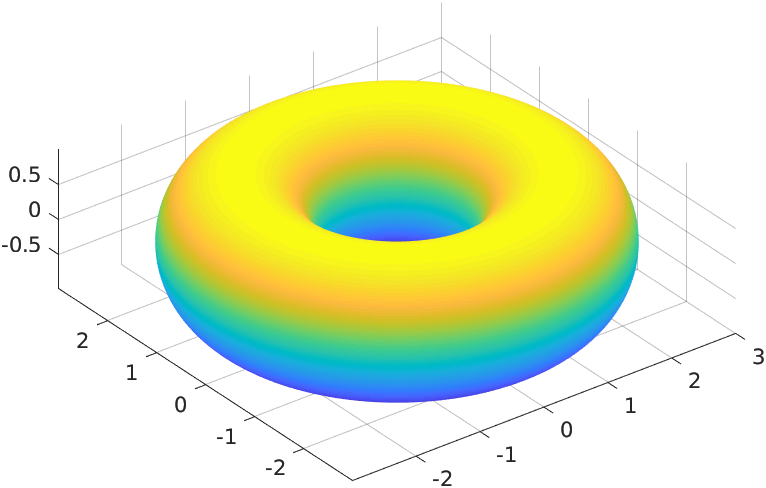
\includegraphics[width=0.5\textwidth]{img/e16p1.png}
\end{center}
\end{solution}